% Generated by Sphinx.
\def\sphinxdocclass{report}
\documentclass[a4paper,10pt,english]{sphinxmanual}
\usepackage[utf8]{inputenc}
\DeclareUnicodeCharacter{00A0}{\nobreakspace}
\usepackage[T1]{fontenc}
\usepackage{babel}
\usepackage{times}
\usepackage[Bjarne]{fncychap}
\usepackage{longtable}
\usepackage{sphinx}
\usepackage{multirow}


\title{A Little Book of R For Bayesian Statistics}
\date{April 22, 2013}
\release{0.1}
\author{Avril Coghlan}
\newcommand{\sphinxlogo}{}
\renewcommand{\releasename}{Release}
\makeindex

\makeatletter
\def\PYG@reset{\let\PYG@it=\relax \let\PYG@bf=\relax%
    \let\PYG@ul=\relax \let\PYG@tc=\relax%
    \let\PYG@bc=\relax \let\PYG@ff=\relax}
\def\PYG@tok#1{\csname PYG@tok@#1\endcsname}
\def\PYG@toks#1+{\ifx\relax#1\empty\else%
    \PYG@tok{#1}\expandafter\PYG@toks\fi}
\def\PYG@do#1{\PYG@bc{\PYG@tc{\PYG@ul{%
    \PYG@it{\PYG@bf{\PYG@ff{#1}}}}}}}
\def\PYG#1#2{\PYG@reset\PYG@toks#1+\relax+\PYG@do{#2}}

\def\PYG@tok@gd{\def\PYG@tc##1{\textcolor[rgb]{0.63,0.00,0.00}{##1}}}
\def\PYG@tok@gu{\let\PYG@bf=\textbf\def\PYG@tc##1{\textcolor[rgb]{0.50,0.00,0.50}{##1}}}
\def\PYG@tok@gt{\def\PYG@tc##1{\textcolor[rgb]{0.00,0.25,0.82}{##1}}}
\def\PYG@tok@gs{\let\PYG@bf=\textbf}
\def\PYG@tok@gr{\def\PYG@tc##1{\textcolor[rgb]{1.00,0.00,0.00}{##1}}}
\def\PYG@tok@cm{\let\PYG@it=\textit\def\PYG@tc##1{\textcolor[rgb]{0.25,0.50,0.56}{##1}}}
\def\PYG@tok@vg{\def\PYG@tc##1{\textcolor[rgb]{0.73,0.38,0.84}{##1}}}
\def\PYG@tok@m{\def\PYG@tc##1{\textcolor[rgb]{0.13,0.50,0.31}{##1}}}
\def\PYG@tok@mh{\def\PYG@tc##1{\textcolor[rgb]{0.13,0.50,0.31}{##1}}}
\def\PYG@tok@cs{\def\PYG@tc##1{\textcolor[rgb]{0.25,0.50,0.56}{##1}}\def\PYG@bc##1{\colorbox[rgb]{1.00,0.94,0.94}{##1}}}
\def\PYG@tok@ge{\let\PYG@it=\textit}
\def\PYG@tok@vc{\def\PYG@tc##1{\textcolor[rgb]{0.73,0.38,0.84}{##1}}}
\def\PYG@tok@il{\def\PYG@tc##1{\textcolor[rgb]{0.13,0.50,0.31}{##1}}}
\def\PYG@tok@go{\def\PYG@tc##1{\textcolor[rgb]{0.19,0.19,0.19}{##1}}}
\def\PYG@tok@cp{\def\PYG@tc##1{\textcolor[rgb]{0.00,0.44,0.13}{##1}}}
\def\PYG@tok@gi{\def\PYG@tc##1{\textcolor[rgb]{0.00,0.63,0.00}{##1}}}
\def\PYG@tok@gh{\let\PYG@bf=\textbf\def\PYG@tc##1{\textcolor[rgb]{0.00,0.00,0.50}{##1}}}
\def\PYG@tok@ni{\let\PYG@bf=\textbf\def\PYG@tc##1{\textcolor[rgb]{0.84,0.33,0.22}{##1}}}
\def\PYG@tok@nl{\let\PYG@bf=\textbf\def\PYG@tc##1{\textcolor[rgb]{0.00,0.13,0.44}{##1}}}
\def\PYG@tok@nn{\let\PYG@bf=\textbf\def\PYG@tc##1{\textcolor[rgb]{0.05,0.52,0.71}{##1}}}
\def\PYG@tok@no{\def\PYG@tc##1{\textcolor[rgb]{0.38,0.68,0.84}{##1}}}
\def\PYG@tok@na{\def\PYG@tc##1{\textcolor[rgb]{0.25,0.44,0.63}{##1}}}
\def\PYG@tok@nb{\def\PYG@tc##1{\textcolor[rgb]{0.00,0.44,0.13}{##1}}}
\def\PYG@tok@nc{\let\PYG@bf=\textbf\def\PYG@tc##1{\textcolor[rgb]{0.05,0.52,0.71}{##1}}}
\def\PYG@tok@nd{\let\PYG@bf=\textbf\def\PYG@tc##1{\textcolor[rgb]{0.33,0.33,0.33}{##1}}}
\def\PYG@tok@ne{\def\PYG@tc##1{\textcolor[rgb]{0.00,0.44,0.13}{##1}}}
\def\PYG@tok@nf{\def\PYG@tc##1{\textcolor[rgb]{0.02,0.16,0.49}{##1}}}
\def\PYG@tok@si{\let\PYG@it=\textit\def\PYG@tc##1{\textcolor[rgb]{0.44,0.63,0.82}{##1}}}
\def\PYG@tok@s2{\def\PYG@tc##1{\textcolor[rgb]{0.25,0.44,0.63}{##1}}}
\def\PYG@tok@vi{\def\PYG@tc##1{\textcolor[rgb]{0.73,0.38,0.84}{##1}}}
\def\PYG@tok@nt{\let\PYG@bf=\textbf\def\PYG@tc##1{\textcolor[rgb]{0.02,0.16,0.45}{##1}}}
\def\PYG@tok@nv{\def\PYG@tc##1{\textcolor[rgb]{0.73,0.38,0.84}{##1}}}
\def\PYG@tok@s1{\def\PYG@tc##1{\textcolor[rgb]{0.25,0.44,0.63}{##1}}}
\def\PYG@tok@gp{\let\PYG@bf=\textbf\def\PYG@tc##1{\textcolor[rgb]{0.78,0.36,0.04}{##1}}}
\def\PYG@tok@sh{\def\PYG@tc##1{\textcolor[rgb]{0.25,0.44,0.63}{##1}}}
\def\PYG@tok@ow{\let\PYG@bf=\textbf\def\PYG@tc##1{\textcolor[rgb]{0.00,0.44,0.13}{##1}}}
\def\PYG@tok@sx{\def\PYG@tc##1{\textcolor[rgb]{0.78,0.36,0.04}{##1}}}
\def\PYG@tok@bp{\def\PYG@tc##1{\textcolor[rgb]{0.00,0.44,0.13}{##1}}}
\def\PYG@tok@c1{\let\PYG@it=\textit\def\PYG@tc##1{\textcolor[rgb]{0.25,0.50,0.56}{##1}}}
\def\PYG@tok@kc{\let\PYG@bf=\textbf\def\PYG@tc##1{\textcolor[rgb]{0.00,0.44,0.13}{##1}}}
\def\PYG@tok@c{\let\PYG@it=\textit\def\PYG@tc##1{\textcolor[rgb]{0.25,0.50,0.56}{##1}}}
\def\PYG@tok@mf{\def\PYG@tc##1{\textcolor[rgb]{0.13,0.50,0.31}{##1}}}
\def\PYG@tok@err{\def\PYG@bc##1{\fcolorbox[rgb]{1.00,0.00,0.00}{1,1,1}{##1}}}
\def\PYG@tok@kd{\let\PYG@bf=\textbf\def\PYG@tc##1{\textcolor[rgb]{0.00,0.44,0.13}{##1}}}
\def\PYG@tok@ss{\def\PYG@tc##1{\textcolor[rgb]{0.32,0.47,0.09}{##1}}}
\def\PYG@tok@sr{\def\PYG@tc##1{\textcolor[rgb]{0.14,0.33,0.53}{##1}}}
\def\PYG@tok@mo{\def\PYG@tc##1{\textcolor[rgb]{0.13,0.50,0.31}{##1}}}
\def\PYG@tok@mi{\def\PYG@tc##1{\textcolor[rgb]{0.13,0.50,0.31}{##1}}}
\def\PYG@tok@kn{\let\PYG@bf=\textbf\def\PYG@tc##1{\textcolor[rgb]{0.00,0.44,0.13}{##1}}}
\def\PYG@tok@o{\def\PYG@tc##1{\textcolor[rgb]{0.40,0.40,0.40}{##1}}}
\def\PYG@tok@kr{\let\PYG@bf=\textbf\def\PYG@tc##1{\textcolor[rgb]{0.00,0.44,0.13}{##1}}}
\def\PYG@tok@s{\def\PYG@tc##1{\textcolor[rgb]{0.25,0.44,0.63}{##1}}}
\def\PYG@tok@kp{\def\PYG@tc##1{\textcolor[rgb]{0.00,0.44,0.13}{##1}}}
\def\PYG@tok@w{\def\PYG@tc##1{\textcolor[rgb]{0.73,0.73,0.73}{##1}}}
\def\PYG@tok@kt{\def\PYG@tc##1{\textcolor[rgb]{0.56,0.13,0.00}{##1}}}
\def\PYG@tok@sc{\def\PYG@tc##1{\textcolor[rgb]{0.25,0.44,0.63}{##1}}}
\def\PYG@tok@sb{\def\PYG@tc##1{\textcolor[rgb]{0.25,0.44,0.63}{##1}}}
\def\PYG@tok@k{\let\PYG@bf=\textbf\def\PYG@tc##1{\textcolor[rgb]{0.00,0.44,0.13}{##1}}}
\def\PYG@tok@se{\let\PYG@bf=\textbf\def\PYG@tc##1{\textcolor[rgb]{0.25,0.44,0.63}{##1}}}
\def\PYG@tok@sd{\let\PYG@it=\textit\def\PYG@tc##1{\textcolor[rgb]{0.25,0.44,0.63}{##1}}}

\def\PYGZbs{\char`\\}
\def\PYGZus{\char`\_}
\def\PYGZob{\char`\{}
\def\PYGZcb{\char`\}}
\def\PYGZca{\char`\^}
\def\PYGZsh{\char`\#}
\def\PYGZpc{\char`\%}
\def\PYGZdl{\char`\$}
\def\PYGZti{\char`\~}
% for compatibility with earlier versions
\def\PYGZat{@}
\def\PYGZlb{[}
\def\PYGZrb{]}
\makeatother

\begin{document}

\maketitle
\tableofcontents
\phantomsection\label{index::doc}


By \href{http://www.sanger.ac.uk/research/projects/parasitegenomics/}{Avril Coghlan},
Wellcome Trust Sanger Institute, Cambridge, U.K.
Email: \href{mailto:alc@sanger.ac.uk}{alc@sanger.ac.uk}

This is a simple introduction to Bayesian statistics using the R statistics software.

There is a pdf version of this booklet available at:
\href{https://github.com/avrilcoghlan/LittleBookofRBayesianStatistics/raw/master/\_build/latex/BayesianStats.pdf}{https://github.com/avrilcoghlan/LittleBookofRBayesianStatistics/raw/master/\_build/latex/BayesianStats.pdf}.

If you like this booklet, you may also like to check out my booklets on using
R for biomedical statistics,
\href{http://a-little-book-of-r-for-biomedical-statistics.readthedocs.org/}{http://a-little-book-of-r-for-biomedical-statistics.readthedocs.org/},
using R for time series analysis,
\href{http://a-little-book-of-r-for-time-series.readthedocs.org/}{http://a-little-book-of-r-for-time-series.readthedocs.org/}, and
using R for multivariate analysis,
\href{http://little-book-of-r-for-multivariate-analysis.readthedocs.org/}{http://little-book-of-r-for-multivariate-analysis.readthedocs.org/}.

Contents:


\chapter{How to install R}
\label{src/installr:welcome-to-a-little-book-of-r-for-bayesian-statistics}\label{src/installr:how-to-install-r}\label{src/installr::doc}

\section{Introduction to R}
\label{src/installr:introduction-to-r}
This little booklet has some information on how to use R for time series analysis.

R (\href{http://www.r-project.org/}{www.r-project.org}) is a commonly used
free Statistics software. R allows you to carry out statistical
analyses in an interactive mode, as well as allowing simple programming.


\section{Installing R}
\label{src/installr:installing-r}
To use R, you first need to install the R program on your computer.


\subsection{How to check if R is installed on a Windows PC}
\label{src/installr:how-to-check-if-r-is-installed-on-a-windows-pc}
Before you install R on your computer, the first thing to do is to check whether
R is already installed on your computer (for example, by a previous user).

These instructions will focus on installing R on a Windows PC. However, I will also
briefly mention how to install R on a Macintosh or Linux computer (see below).

If you are using a Windows PC, there are two ways you can check whether R is
already isntalled on your computer:
\begin{enumerate}
\item {} 
Check if there is an ``R'' icon on the desktop of the computer that you are using.
If so, double-click on the ``R'' icon to start R. If you cannot find an ``R'' icon, try step 2 instead.

\item {} 
Click on the ``Start'' menu at the bottom left of your Windows desktop, and then move your
mouse over ``All Programs'' in the menu that pops up. See if ``R'' appears in the list
of programs that pops up. If it does, it means that R is already installed on your
computer, and you can start R by selecting ``R''  (or R X.X.X, where X.X.X gives the version of R,
eg. R 2.10.0) from the list.

\end{enumerate}

If either (1) or (2) above does succeed in starting R, it means that R is already installed
on the computer that you are using. (If neither succeeds, R is not installed yet).
If there is an old version of R installed on the Windows PC that you are using,
it is worth installing the latest version of R, to make sure that you have all the
latest R functions available to you to use.


\subsection{Finding out what is the latest version of R}
\label{src/installr:finding-out-what-is-the-latest-version-of-r}
To find out what is the latest version of R, you can look at the CRAN (Comprehensive
R Network) website, \href{http://cran.r-project.org/}{http://cran.r-project.org/}.

Beside ``The latest release'' (about half way down the page), it will say something like
``R-X.X.X.tar.gz'' (eg. ``R-2.12.1.tar.gz''). This means that the latest release of R is X.X.X (for
example, 2.12.1).

New releases of R are made very regularly (approximately once a month), as R is actively being
improved all the time. It is worthwhile installing new versions of R regularly, to make sure
that you have a recent version of R (to ensure compatibility with all the latest versions of
the R packages that you have downloaded).


\subsection{Installing R on a Windows PC}
\label{src/installr:installing-r-on-a-windows-pc}
To install R on your Windows computer, follow these steps:
\begin{enumerate}
\item {} 
Go to \href{http://ftp.heanet.ie/mirrors/cran.r-project.org}{http://ftp.heanet.ie/mirrors/cran.r-project.org}.

\item {} 
Under ``Download and Install R'', click on the ``Windows'' link.

\item {} 
Under ``Subdirectories'', click on the ``base'' link.

\item {} 
On the next page, you should see a link saying something like ``Download R 2.10.1 for Windows'' (or R X.X.X, where X.X.X gives the version of R, eg. R 2.11.1).
Click on this link.

\item {} 
You may be asked if you want to save or run a file ``R-2.10.1-win32.exe''. Choose ``Save'' and
save the file on the Desktop. Then double-click on the icon for the file to run it.

\item {} 
You will be asked what language to install it in - choose English.

\item {} 
The R Setup Wizard will appear in a window. Click ``Next'' at the bottom of the R Setup wizard
window.

\item {} 
The next page says ``Information'' at the top. Click ``Next'' again.

\item {} 
The next page says ``Information'' at the top. Click ``Next'' again.

\item {} 
The next page says ``Select Destination Location'' at the top.
By default, it will suggest to install R in ``C:\textbackslash{}Program Files'' on your computer.

\item {} 
Click ``Next'' at the bottom of the R Setup wizard window.

\item {} 
The next page says ``Select components'' at the top. Click ``Next'' again.

\item {} 
The next page says ``Startup options'' at the top. Click ``Next'' again.

\item {} 
The next page says ``Select start menu folder'' at the top. Click ``Next'' again.

\item {} 
The next page says ``Select additional tasks'' at the top. Click ``Next'' again.

\item {} 
R should now be installed. This will take about a minute. When R has finished, you will
see ``Completing the R for Windows Setup Wizard'' appear. Click ``Finish''.

\item {} 
To start R, you can either follow step 18, or 19:

\item {} 
Check if there is an ``R'' icon on the desktop of the computer that you are using.
If so, double-click on the ``R'' icon to start R. If you cannot find an ``R'' icon, try step 19 instead.

\item {} 
Click on the ``Start'' button at the bottom left of your computer screen, and then
choose ``All programs'', and start R by selecting ``R''  (or R X.X.X, where
X.X.X gives the version of R, eg. R 2.10.0) from the menu of programs.

\item {} 
The R console (a rectangle) should pop up:

\end{enumerate}

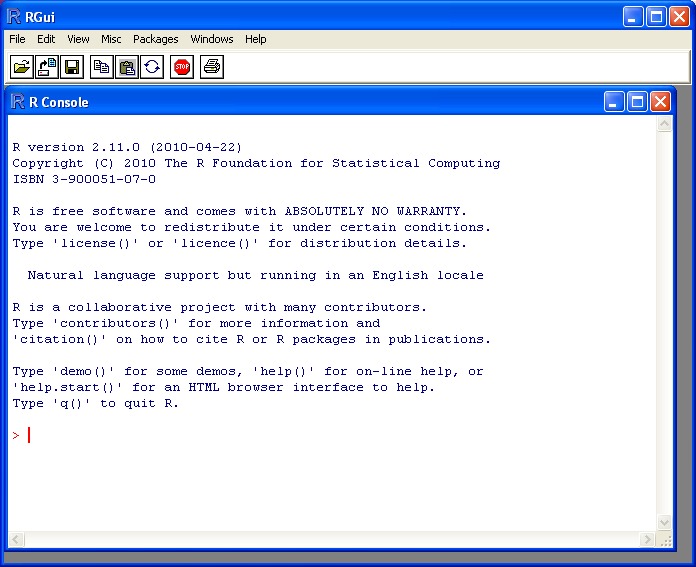
\includegraphics{image3.png}


\subsection{How to install R on non-Windows computers (eg. Macintosh or Linux computers)}
\label{src/installr:how-to-install-r-on-non-windows-computers-eg-macintosh-or-linux-computers}
The instructions above are for installing R on a Windows PC. If you want to install R
on a computer that has a non-Windows operating system (for example, a Macintosh or computer running Linux,
you should download the appropriate R installer for that operating system at
\href{http://ftp.heanet.ie/mirrors/cran.r-project.org/}{http://ftp.heanet.ie/mirrors/cran.r-project.org} and
follow the R installation instructions for the appropriate operating system at
\href{http://ftp.heanet.ie/mirrors/cran.r-project.org/doc/FAQ/R-FAQ.html\#How-can-R-be-installed\_003f}{http://ftp.heanet.ie/mirrors/cran.r-project.org/doc/FAQ/R-FAQ.html\#How-can-R-be-installed\_003f}).


\section{Installing R packages}
\label{src/installr:installing-r-packages}
R comes with some standard packages that are installed when you install R. However, in this
booklet I will also tell you how to use some additional R packages that are useful, for example,
the ``rmeta'' package. These additional packages do not come with the standard installation of R,
so you need to install them yourself.


\subsection{How to install an R package}
\label{src/installr:how-to-install-an-r-package}
Once you have installed R on a Windows computer (following the steps above), you can install
an additional package by following the steps below:
\begin{enumerate}
\item {} 
To start R, follow either step 2 or 3:

\item {} 
Check if there is an ``R'' icon on the desktop of the computer that you are using.
If so, double-click on the ``R'' icon to start R. If you cannot find an ``R'' icon, try step 3 instead.

\item {} 
Click on the ``Start'' button at the bottom left of your computer screen, and then
choose ``All programs'', and start R by selecting ``R''  (or R X.X.X, where
X.X.X gives the version of R, eg. R 2.10.0) from the menu of programs.

\item {} 
The R console (a rectangle) should pop up.

\item {} 
Once you have started R, you can now install an R package (eg. the ``rmeta'' package) by
choosing ``Install package(s)'' from the ``Packages'' menu at the top of the R console.
This will ask you what website you want to download the package from, you should choose
``Ireland'' (or another country, if you prefer). It will also bring up a list of available
packages that you can install, and you should choose the package that you want to install
from that list (eg. ``rmeta'').

\item {} 
This will install the ``rmeta'' package.

\item {} 
The ``rmeta'' package is now installed. Whenever you want to use the ``rmeta'' package after this,
after starting R, you first have to load the package by typing into the R console:

\end{enumerate}

\begin{Verbatim}[commandchars=\\\{\}]
\PYG{o}{\textgreater{}} library\PYG{p}{(}\PYG{l+s}{"}\PYG{l+s}{rmeta"}\PYG{p}{)}
\end{Verbatim}

Note that there are some additional R packages for bioinformatics that are part of a special
set of R packages called Bioconductor (\href{http://www.bioconductor.org/}{www.bioconductor.org})
such as the ``yeastExpData'' R package, the ``Biostrings'' R package, etc.).
These Bioconductor packages need to be installed using a different, Bioconductor-specific procedure
(see {\hyperref[src/installr:how-to-install-a-bioconductor-r-package]{How to install a Bioconductor R package}} below).


\subsection{How to install a Bioconductor R package}
\label{src/installr:how-to-install-a-bioconductor-r-package}
The procedure above can be used to install the majority of R packages. However, the
Bioconductor set of bioinformatics R packages need to be installed by a special procedure.
Bioconductor (\href{http://www.bioconductor.org/}{www.bioconductor.org})
is a group of R packages that have been developed for bioinformatics. This includes
R packages such as ``yeastExpData'', ``Biostrings'', etc.

To install the Bioconductor packages, follow these steps:
\begin{enumerate}
\item {} 
To start R, follow either step 2 or 3:

\item {} 
Check if there is an ``R'' icon on the desktop of the computer that you are using.
If so, double-click on the ``R'' icon to start R. If you cannot find an ``R'' icon, try step 3 instead.

\item {} 
Click on the ``Start'' button at the bottom left of your computer screen, and then choose ``All programs'', and start R by selecting ``R''  (or R X.X.X, where X.X.X gives the version of R, eg. R 2.10.0) from the menu of programs.

\item {} 
The R console (a rectangle) should pop up.

\item {} 
Once you have started R, now type in the R console:

\end{enumerate}

\begin{Verbatim}[commandchars=\\\{\}]
\PYG{o}{\textgreater{}} source\PYG{p}{(}\PYG{l+s}{"}\PYG{l+s}{http://bioconductor.org/biocLite.R"}\PYG{p}{)}
\PYG{o}{\textgreater{}} biocLite\PYG{p}{(}\PYG{p}{)}
\end{Verbatim}
\begin{enumerate}
\setcounter{enumi}{5}
\item {} 
This will install a core set of Bioconductor packages (``affy'', ``affydata'', ``affyPLM'',
``annaffy'', ``annotate'', ``Biobase'', ``Biostrings'', ``DynDoc'', ``gcrma'', ``genefilter'',
``geneplotter'', ``hgu95av2.db'', ``limma'', ``marray'', ``matchprobes'', ``multtest'', ``ROC'',
``vsn'', ``xtable'', ``affyQCReport'').
This takes a few minutes (eg. 10 minutes).

\item {} 
At a later date, you may wish to install some extra Bioconductor packages that do not belong
to the core set of Bioconductor packages. For example, to install the Bioconductor package called
``yeastExpData'', start R and type in the R console:

\end{enumerate}

\begin{Verbatim}[commandchars=\\\{\}]
\PYG{o}{\textgreater{}} source\PYG{p}{(}\PYG{l+s}{"}\PYG{l+s}{http://bioconductor.org/biocLite.R"}\PYG{p}{)}
\PYG{o}{\textgreater{}} biocLite\PYG{p}{(}\PYG{l+s}{"}\PYG{l+s}{yeastExpData"}\PYG{p}{)}
\end{Verbatim}
\begin{enumerate}
\setcounter{enumi}{7}
\item {} 
Whenever you want to use a package after installing it, you need to load it into R by typing:

\end{enumerate}

\begin{Verbatim}[commandchars=\\\{\}]
\PYG{o}{\textgreater{}} library\PYG{p}{(}\PYG{l+s}{"}\PYG{l+s}{yeastExpData"}\PYG{p}{)}
\end{Verbatim}


\section{Running R}
\label{src/installr:running-r}
To use R, you first need to start the R program on your computer.
You should have already installed R on your computer (see above).

To start R, you can either follow step 1 or 2:
1. Check if there is an ``R'' icon on the desktop of the computer that you are using.
\begin{quote}

If so, double-click on the ``R'' icon to start R. If you cannot find an ``R'' icon, try step 2 instead.
\end{quote}
\begin{enumerate}
\setcounter{enumi}{1}
\item {} 
Click on the ``Start'' button at the bottom left of your computer screen, and then choose ``All programs'', and start R by selecting ``R''  (or R X.X.X, where X.X.X gives the version of R, eg. R 2.10.0) from the menu of programs.

\end{enumerate}

This should bring up a new window, which is the \emph{R console}.


\section{A brief introduction to R}
\label{src/installr:a-brief-introduction-to-r}
You will type R commands into the R console in order to carry out
analyses in R. In the R console you will see:

\begin{Verbatim}[commandchars=\\\{\}]
\PYG{o}{\textgreater{}}
\end{Verbatim}

This is the R prompt. We type the commands needed for a particular
task after this prompt. The command is carried out after you hit
the Return key.

Once you have started R, you can start typing in commands, and the
results will be calculated immediately, for example:

\begin{Verbatim}[commandchars=\\\{\}]
\PYG{o}{\textgreater{}} \PYG{l+m}{2}\PYG{o}{*}\PYG{l+m}{3}
\PYG{p}{[}\PYG{l+m}{1}\PYG{p}{]} \PYG{l+m}{6}
\PYG{o}{\textgreater{}} \PYG{l+m}{10}\PYG{o}{-}\PYG{l+m}{3}
\PYG{p}{[}\PYG{l+m}{1}\PYG{p}{]} \PYG{l+m}{7}
\end{Verbatim}

All variables (scalars, vectors, matrices, etc.) created by R are
called \emph{objects}. In R, we assign values to variables using an
arrow. For example, we can assign the value 2*3 to the variable
\emph{x} using the command:

\begin{Verbatim}[commandchars=\\\{\}]
\PYG{o}{\textgreater{}} x \PYG{o}{\textless{}-} \PYG{l+m}{2}\PYG{o}{*}\PYG{l+m}{3}
\end{Verbatim}

To view the contents of any R object, just type its name, and the
contents of that R object will be displayed:

\begin{Verbatim}[commandchars=\\\{\}]
\PYG{o}{\textgreater{}} x
\PYG{p}{[}\PYG{l+m}{1}\PYG{p}{]} \PYG{l+m}{6}
\end{Verbatim}

There are several possible different types of objects in R,
including scalars, vectors, matrices, arrays, data frames, tables,
and lists. The scalar variable \emph{x} above is one example of an R
object. While a scalar variable such as \emph{x} has just one element, a
vector consists of several elements. The elements in a vector are
all of the same type (eg. numeric or characters), while lists may
include elements such as characters as well as numeric quantities.

To create a vector, we can use the c() (combine) function. For
example, to create a vector called \emph{myvector} that has elements
with values 8, 6, 9, 10, and 5, we type:

\begin{Verbatim}[commandchars=\\\{\}]
\PYG{o}{\textgreater{}} myvector \PYG{o}{\textless{}-} c\PYG{p}{(}\PYG{l+m}{8}\PYG{p}{,} \PYG{l+m}{6}\PYG{p}{,} \PYG{l+m}{9}\PYG{p}{,} \PYG{l+m}{10}\PYG{p}{,} \PYG{l+m}{5}\PYG{p}{)}
\end{Verbatim}

To see the contents of the variable \emph{myvector}, we can just type
its name:

\begin{Verbatim}[commandchars=\\\{\}]
\PYG{o}{\textgreater{}} myvector
\PYG{p}{[}\PYG{l+m}{1}\PYG{p}{]}  \PYG{l+m}{8}  \PYG{l+m}{6}  \PYG{l+m}{9} \PYG{l+m}{10}  \PYG{l+m}{5}
\end{Verbatim}

The {[}1{]} is the index of the first element in the vector. We can
extract any element of the vector by typing the vector name with
the index of that element given in square brackets. For example, to
get the value of the 4th element in the vector \emph{myvector}, we
type:

\begin{Verbatim}[commandchars=\\\{\}]
\PYG{o}{\textgreater{}} myvector\PYG{p}{[}\PYG{l+m}{4}\PYG{p}{]}
\PYG{p}{[}\PYG{l+m}{1}\PYG{p}{]} \PYG{l+m}{10}
\end{Verbatim}

In contrast to a vector, a list can contain elements of different
types, for example, both numeric and character elements. A list can
also include other variables such as a vector. The list() function
is used to create a list. For example, we could create a list
\emph{mylist} by typing:

\begin{Verbatim}[commandchars=\\\{\}]
\PYG{o}{\textgreater{}} mylist \PYG{o}{\textless{}-} list\PYG{p}{(}name\PYG{o}{=}\PYG{l+s}{"}\PYG{l+s}{Fred"}\PYG{p}{,} wife\PYG{o}{=}\PYG{l+s}{"}\PYG{l+s}{Mary"}\PYG{p}{,} myvector\PYG{p}{)}
\end{Verbatim}

We can then print out the contents of the list \emph{mylist} by typing
its name:

\begin{Verbatim}[commandchars=\\\{\}]
\PYG{o}{\textgreater{}} mylist
\PYG{p}{\PYGZdl{}}name
\PYG{p}{[}\PYG{l+m}{1}\PYG{p}{]} \PYG{l+s}{"}\PYG{l+s}{Fred"}

\PYG{p}{\PYGZdl{}}wife
\PYG{p}{[}\PYG{l+m}{1}\PYG{p}{]} \PYG{l+s}{"}\PYG{l+s}{Mary"}

\PYG{p}{[}\PYG{p}{[}\PYG{l+m}{3}\PYG{p}{]}\PYG{p}{]}
\PYG{p}{[}\PYG{l+m}{1}\PYG{p}{]}  \PYG{l+m}{8}  \PYG{l+m}{6}  \PYG{l+m}{9} \PYG{l+m}{10}  \PYG{l+m}{5}
\end{Verbatim}

The elements in a list are numbered, and can be referred to using
indices. We can extract an element of a list by typing the list
name with the index of the element given in double square brackets
(in contrast to a vector, where we only use single square
brackets). Thus, we can extract the second and third elements from
\emph{mylist} by typing:

\begin{Verbatim}[commandchars=\\\{\}]
\PYG{o}{\textgreater{}} mylist\PYG{p}{[}\PYG{p}{[}\PYG{l+m}{2}\PYG{p}{]}\PYG{p}{]}
\PYG{p}{[}\PYG{l+m}{1}\PYG{p}{]} \PYG{l+s}{"}\PYG{l+s}{Mary"}
\PYG{o}{\textgreater{}} mylist\PYG{p}{[}\PYG{p}{[}\PYG{l+m}{3}\PYG{p}{]}\PYG{p}{]}
\PYG{p}{[}\PYG{l+m}{1}\PYG{p}{]}  \PYG{l+m}{8}  \PYG{l+m}{6}  \PYG{l+m}{9} \PYG{l+m}{10}  \PYG{l+m}{5}
\end{Verbatim}

Elements of lists may also be named, and in this case the elements
may be referred to by giving the list name, followed by ``\$'',
followed by the element name. For example, \emph{mylist\$name} is the
same as \emph{mylist{[}{[}1{]}{]}} and \emph{mylist\$wife} is the same as
\emph{mylist{[}{[}2{]}{]}}:

\begin{Verbatim}[commandchars=\\\{\}]
\PYG{o}{\textgreater{}} mylist\PYG{p}{\PYGZdl{}}wife
\PYG{p}{[}\PYG{l+m}{1}\PYG{p}{]} \PYG{l+s}{"}\PYG{l+s}{Mary"}
\end{Verbatim}

We can find out the names of the named elements in a list by using
the attributes() function, for example:

\begin{Verbatim}[commandchars=\\\{\}]
\PYG{o}{\textgreater{}} attributes\PYG{p}{(}mylist\PYG{p}{)}
\PYG{p}{\PYGZdl{}}names
\PYG{p}{[}\PYG{l+m}{1}\PYG{p}{]} \PYG{l+s}{"}\PYG{l+s}{name"} \PYG{l+s}{"}\PYG{l+s}{wife"} \PYG{l+s}{"}\PYG{l+s}{"}
\end{Verbatim}

When you use the attributes() function to find the named elements
of a list variable, the named elements are always listed under a
heading ``\$names''. Therefore, we see that the named elements of the
list variable \emph{mylist} are called ``name'' and ``wife'', and we can
retrieve their values by typing \emph{mylist\$name} and \emph{mylist\$wife},
respectively.

Another type of object that you will encounter in R is a \emph{table}
variable. For example, if we made a vector variable \emph{mynames}
containing the names of children in a class, we can use the table()
function to produce a table variable that contains the number of
children with each possible name:

\begin{Verbatim}[commandchars=\\\{\}]
\PYG{o}{\textgreater{}} mynames \PYG{o}{\textless{}-} c\PYG{p}{(}\PYG{l+s}{"}\PYG{l+s}{Mary"}\PYG{p}{,} \PYG{l+s}{"}\PYG{l+s}{John"}\PYG{p}{,} \PYG{l+s}{"}\PYG{l+s}{Ann"}\PYG{p}{,} \PYG{l+s}{"}\PYG{l+s}{Sinead"}\PYG{p}{,} \PYG{l+s}{"}\PYG{l+s}{Joe"}\PYG{p}{,} \PYG{l+s}{"}\PYG{l+s}{Mary"}\PYG{p}{,} \PYG{l+s}{"}\PYG{l+s}{Jim"}\PYG{p}{,} \PYG{l+s}{"}\PYG{l+s}{John"}\PYG{p}{,} \PYG{l+s}{"}\PYG{l+s}{Simon"}\PYG{p}{)}
\PYG{o}{\textgreater{}} table\PYG{p}{(}mynames\PYG{p}{)}
mynames
   Ann    Jim    Joe   John   Mary  Simon Sinead
     \PYG{l+m}{1}      \PYG{l+m}{1}      \PYG{l+m}{1}      \PYG{l+m}{2}      \PYG{l+m}{2}      \PYG{l+m}{1}      \PYG{l+m}{1}
\end{Verbatim}

We can store the table variable produced by the function table(),
and call the stored table ``mytable'', by typing:

\begin{Verbatim}[commandchars=\\\{\}]
\PYG{o}{\textgreater{}} mytable \PYG{o}{\textless{}-} table\PYG{p}{(}mynames\PYG{p}{)}
\end{Verbatim}

To access elements in a table variable, you need to use double
square brackets, just like accessing elements in a list. For
example, to access the fourth element in the table \emph{mytable} (the
number of children called ``John''), we type:

\begin{Verbatim}[commandchars=\\\{\}]
\PYG{o}{\textgreater{}} mytable\PYG{p}{[}\PYG{p}{[}\PYG{l+m}{4}\PYG{p}{]}\PYG{p}{]}
\PYG{p}{[}\PYG{l+m}{1}\PYG{p}{]} \PYG{l+m}{2}
\end{Verbatim}

Alternatively, you can use the name of the fourth element in
the table (``John'') to find the value of that table element:

\begin{Verbatim}[commandchars=\\\{\}]
\PYG{o}{\textgreater{}} mytable\PYG{p}{[}\PYG{p}{[}\PYG{l+s}{"}\PYG{l+s}{John"}\PYG{p}{]}\PYG{p}{]}
\PYG{p}{[}\PYG{l+m}{1}\PYG{p}{]} \PYG{l+m}{2}
\end{Verbatim}

Functions in R usually require \emph{arguments}, which are input
variables (ie. objects) that are passed to them, which they then
carry out some operation on. For example, the log10() function is
passed a number, and it then calculates the log to the base 10 of
that number:

\begin{Verbatim}[commandchars=\\\{\}]
\PYG{o}{\textgreater{}} log10\PYG{p}{(}\PYG{l+m}{100}\PYG{p}{)}
\PYG{l+m}{2}
\end{Verbatim}

In R, you can get help about a particular function by using the
help() function. For example, if you want help about the log10()
function, you can type:

\begin{Verbatim}[commandchars=\\\{\}]
\PYG{o}{\textgreater{}} help\PYG{p}{(}\PYG{l+s}{"}\PYG{l+s}{log10"}\PYG{p}{)}
\end{Verbatim}

When you use the help() function, a box or webpage will pop up with
information about the function that you asked for help with.

If you are not sure of the name of a function, but think you know
part of its name, you can search for the function name using the
help.search() and RSiteSearch() functions. The help.search() function
searches to see if you already have a function installed (from one of
the R packages that you have installed) that may be related to some
topic you're interested in. The RSiteSearch() function searches all
R functions (including those in packages that you haven't yet installed)
for functions related to the topic you are interested in.

For example, if you want to know if there
is a function to calculate the standard deviation of a set of
numbers, you can search for the names of all installed functions containing
the word ``deviation'' in their description by typing:

\begin{Verbatim}[commandchars=\\\{\}]
\PYG{o}{\textgreater{}} help.search\PYG{p}{(}\PYG{l+s}{"}\PYG{l+s}{deviation"}\PYG{p}{)}
Help files with alias or concept or title matching
\PYG{l+s}{'}\PYG{l+s}{deviation'} using fuzzy matching:

genefilter\PYG{p}{::}rowSds
                    Row variance and standard deviation of
                    a numeric array
nlme\PYG{p}{::}pooledSD      Extract Pooled Standard Deviation
stats\PYG{p}{::}mad          Median Absolute Deviation
stats\PYG{p}{::}sd           Standard Deviation
vsn\PYG{p}{::}meanSdPlot     Plot row standard deviations versus row
\end{Verbatim}

Among the functions that were found, is the function sd() in the
``stats'' package (an R package that comes with the standard R
installation), which is used for calculating the standard deviation.

In the example above, the help.search() function found a relevant
function (sd() here). However, if you did not find what you were looking
for with help.search(), you could then use the RSiteSearch() function to
see if a search of all functions described on the R website may find
something relevant to the topic that you're interested in:

\begin{Verbatim}[commandchars=\\\{\}]
\PYG{o}{\textgreater{}} RSiteSearch\PYG{p}{(}\PYG{l+s}{"}\PYG{l+s}{deviation"}\PYG{p}{)}
\end{Verbatim}

The results of the RSiteSearch() function will be hits to descriptions
of R functions, as well as to R mailing list discussions of those
functions.

We can perform computations with R using objects such as scalars
and vectors. For example, to calculate the average of the values in
the vector \emph{myvector} (ie. the average of 8, 6, 9, 10 and 5), we
can use the mean() function:

\begin{Verbatim}[commandchars=\\\{\}]
\PYG{o}{\textgreater{}} mean\PYG{p}{(}myvector\PYG{p}{)}
\PYG{p}{[}\PYG{l+m}{1}\PYG{p}{]} \PYG{l+m}{7.6}
\end{Verbatim}

We have been using built-in R functions such as mean(),
length(), print(), plot(), etc. We can also create our own
functions in R to do calculations that you want to carry out very
often on different input data sets. For example, we can create a
function to calculate the value of 20 plus square of some input
number:

\begin{Verbatim}[commandchars=\\\{\}]
\PYG{o}{\textgreater{}} myfunction \PYG{o}{\textless{}-} \PYG{k+kr}{function}\PYG{p}{(}x\PYG{p}{)} \PYG{p}{\PYGZob{}} \PYG{k+kr}{return}\PYG{p}{(}\PYG{l+m}{20} \PYG{o}{+} \PYG{p}{(}x\PYG{o}{*}x\PYG{p}{)}\PYG{p}{)} \PYG{p}{\PYGZcb{}}
\end{Verbatim}

This function will calculate the square of a number (\emph{x}), and then
add 20 to that value. The return() statement returns the calculated
value. Once you have typed in this function, the function is then
available for use. For example, we can use the function for
different input numbers (eg. 10, 25):

\begin{Verbatim}[commandchars=\\\{\}]
\PYG{o}{\textgreater{}} myfunction\PYG{p}{(}\PYG{l+m}{10}\PYG{p}{)}
\PYG{p}{[}\PYG{l+m}{1}\PYG{p}{]} \PYG{l+m}{120}
\PYG{o}{\textgreater{}} myfunction\PYG{p}{(}\PYG{l+m}{25}\PYG{p}{)}
\PYG{p}{[}\PYG{l+m}{1}\PYG{p}{]} \PYG{l+m}{645}
\end{Verbatim}

To quit R, type:

\begin{Verbatim}[commandchars=\\\{\}]
\PYG{o}{\textgreater{}} q\PYG{p}{(}\PYG{p}{)}
\end{Verbatim}


\section{Links and Further Reading}
\label{src/installr:links-and-further-reading}
Some links are included here for further reading.

For a more in-depth introduction to R, a good online tutorial is
available on the ``Kickstarting R'' website,
\href{http://cran.r-project.org/doc/contrib/Lemon-kickstart/}{cran.r-project.org/doc/contrib/Lemon-kickstart}.

There is another nice (slightly more in-depth) tutorial to R
available on the ``Introduction to R'' website,
\href{http://cran.r-project.org/doc/manuals/R-intro.html}{cran.r-project.org/doc/manuals/R-intro.html}.


\section{Acknowledgements}
\label{src/installr:acknowledgements}
For very helpful comments and suggestions for improvements on the installation instructions, thank you very much to Friedrich Leisch and Phil Spector.


\section{Contact}
\label{src/installr:contact}
I will be very grateful if you will send me (\href{http://www.sanger.ac.uk/research/projects/parasitegenomics/}{Avril Coghlan}) corrections or suggestions for improvements to
my email address \href{mailto:alc@sanger.ac.uk}{alc@sanger.ac.uk}


\section{License}
\label{src/installr:license}
The content in this book is licensed under a \href{http://creativecommons.org/licenses/by/3.0/}{Creative Commons Attribution 3.0 License}.


\chapter{Using R for Bayesian Statistics}
\label{src/bayesianstats::doc}\label{src/bayesianstats:using-r-for-bayesian-statistics}

\section{Bayesian Statistics}
\label{src/bayesianstats:bayesian-statistics}
This booklet tells you how to use the R statistical software to carry out some simple
analyses using Bayesian statistics.

This booklet assumes that the reader has some basic knowledge of Bayesian statistics, and
the principal focus of the booklet is not to explain Bayesian statistics, but rather
to explain how to carry out these analyses using R.

If you are new to Bayesian statistics, and want to learn more about any of the concepts
presented here, I would highly recommend the Open University book
``Bayesian Statistics'' (product code M249/04), available from
from \href{http://www.ouw.co.uk/store/}{the Open University Shop}.

There is a pdf version of this booklet available at
\href{https://github.com/avrilcoghlan/LittleBookofRBayesianStatistics/raw/master/\_build/latex/BayesianStats.pdf}{https://github.com/avrilcoghlan/LittleBookofRBayesianStatistics/ raw/master/\_build/latex/BayesianStats.pdf}.

If you like this booklet, you may also like to check out my booklets on using
R for biomedical statistics,
\href{http://a-little-book-of-r-for-biomedical-statistics.readthedocs.org/}{http://a-little-book-of-r-for-biomedical-statistics.readthedocs.org/},
using R for time series analysis,
\href{http://a-little-book-of-r-for-time-series.readthedocs.org/}{http://a-little-book-of-r-for-time-series.readthedocs.org/},
and using R for multivariate analysis,
\href{http://little-book-of-r-for-multivariate-analysis.readthedocs.org/}{http://little-book-of-r-for-multivariate-analysis.readthedocs.org/}.


\section{Using Bayesian Analysis to Estimate a Proportion}
\label{src/bayesianstats:using-bayesian-analysis-to-estimate-a-proportion}
Bayesian analysis can be useful for estimating a proportion, when you have some rough
idea of what the value of the proportion is, but have relatively little data.


\subsection{Specifying a Prior for a Proportion}
\label{src/bayesianstats:specifying-a-prior-for-a-proportion}
An appropriate prior to use for a proportion is a Beta prior.

For example, if you want to estimate the proportion of people like chocolate, you
might have a rough idea that the most likely value is around 0.85, but that the proportion
is unlikely to be smaller than 0.60 or bigger than 0.95.

You can find the best Beta prior to use in this case by specifying that the median (50\% percentile)
of the prior is 0.85, that the 99.999\% percentile is 0.95, and that the 0.001\% percentile is 0.60:

\begin{Verbatim}[commandchars=\\\{\}]
\PYG{o}{\textgreater{}} quantile1 \PYG{o}{\textless{}-} list\PYG{p}{(}p\PYG{o}{=}\PYG{l+m}{0.5}\PYG{p}{,} x\PYG{o}{=}\PYG{l+m}{0.85}\PYG{p}{)}    \PYG{c+c1}{\PYGZsh{} we believe the median of the prior is 0.85}
\PYG{o}{\textgreater{}} quantile2 \PYG{o}{\textless{}-} list\PYG{p}{(}p\PYG{o}{=}\PYG{l+m}{0.99999}\PYG{p}{,}x\PYG{o}{=}\PYG{l+m}{0.95}\PYG{p}{)} \PYG{c+c1}{\PYGZsh{} we believe the 99.999th percentile of the prior is 0.95}
\PYG{o}{\textgreater{}} quantile3 \PYG{o}{\textless{}-} list\PYG{p}{(}p\PYG{o}{=}\PYG{l+m}{0.00001}\PYG{p}{,}x\PYG{o}{=}\PYG{l+m}{0.60}\PYG{p}{)} \PYG{c+c1}{\PYGZsh{} we believe the 0.001st percentile of the prior is 0.60}
\end{Verbatim}

We can then use the findBeta() function below to find the most appropriate Beta prior to use.

\begin{Verbatim}[commandchars=\\\{\}]
\PYG{o}{\textgreater{}} findBeta \PYG{o}{\textless{}-} \PYG{k+kr}{function}\PYG{p}{(}quantile1\PYG{p}{,}quantile2\PYG{p}{,}quantile3\PYG{p}{)}
  \PYG{p}{\PYGZob{}}
     \PYG{c+c1}{\PYGZsh{} find the quantiles specified by quantile1 and quantile2 and quantile3}
     quantile1\PYGZus{}p \PYG{o}{\textless{}-} quantile1\PYG{p}{[}\PYG{p}{[}\PYG{l+m}{1}\PYG{p}{]}\PYG{p}{]}\PYG{p}{;} quantile1\PYGZus{}q \PYG{o}{\textless{}-} quantile1\PYG{p}{[}\PYG{p}{[}\PYG{l+m}{2}\PYG{p}{]}\PYG{p}{]}
     quantile2\PYGZus{}p \PYG{o}{\textless{}-} quantile2\PYG{p}{[}\PYG{p}{[}\PYG{l+m}{1}\PYG{p}{]}\PYG{p}{]}\PYG{p}{;} quantile2\PYGZus{}q \PYG{o}{\textless{}-} quantile2\PYG{p}{[}\PYG{p}{[}\PYG{l+m}{2}\PYG{p}{]}\PYG{p}{]}
     quantile3\PYGZus{}p \PYG{o}{\textless{}-} quantile3\PYG{p}{[}\PYG{p}{[}\PYG{l+m}{1}\PYG{p}{]}\PYG{p}{]}\PYG{p}{;} quantile3\PYGZus{}q \PYG{o}{\textless{}-} quantile3\PYG{p}{[}\PYG{p}{[}\PYG{l+m}{2}\PYG{p}{]}\PYG{p}{]}

     \PYG{c+c1}{\PYGZsh{} find the beta prior using quantile1 and quantile2}
     priorA \PYG{o}{\textless{}-} beta.select\PYG{p}{(}quantile1\PYG{p}{,}quantile2\PYG{p}{)}
     priorA\PYGZus{}a \PYG{o}{\textless{}-} priorA\PYG{p}{[}\PYG{l+m}{1}\PYG{p}{]}\PYG{p}{;} priorA\PYGZus{}b \PYG{o}{\textless{}-} priorA\PYG{p}{[}\PYG{l+m}{2}\PYG{p}{]}

     \PYG{c+c1}{\PYGZsh{} find the beta prior using quantile1 and quantile3}
     priorB \PYG{o}{\textless{}-} beta.select\PYG{p}{(}quantile1\PYG{p}{,}quantile3\PYG{p}{)}
     priorB\PYGZus{}a \PYG{o}{\textless{}-} priorB\PYG{p}{[}\PYG{l+m}{1}\PYG{p}{]}\PYG{p}{;} priorB\PYGZus{}b \PYG{o}{\textless{}-} priorB\PYG{p}{[}\PYG{l+m}{2}\PYG{p}{]}

     \PYG{c+c1}{\PYGZsh{} find the best possible beta prior}
     diff\PYGZus{}a \PYG{o}{\textless{}-} abs\PYG{p}{(}priorA\PYGZus{}a \PYG{o}{-} priorB\PYGZus{}a\PYG{p}{)}\PYG{p}{;} diff\PYGZus{}b \PYG{o}{\textless{}-} abs\PYG{p}{(}priorB\PYGZus{}b \PYG{o}{-} priorB\PYGZus{}b\PYG{p}{)}
     step\PYGZus{}a \PYG{o}{\textless{}-} diff\PYGZus{}a \PYG{o}{/} \PYG{l+m}{100}\PYG{p}{;} step\PYGZus{}b \PYG{o}{\textless{}-} diff\PYGZus{}b \PYG{o}{/} \PYG{l+m}{100}
     \PYG{k+kr}{if} \PYG{p}{(}priorA\PYGZus{}a \PYG{o}{\textless{}} priorB\PYGZus{}a\PYG{p}{)} \PYG{p}{\PYGZob{}} start\PYGZus{}a \PYG{o}{\textless{}-} priorA\PYGZus{}a\PYG{p}{;} end\PYGZus{}a \PYG{o}{\textless{}-} priorB\PYGZus{}a \PYG{p}{\PYGZcb{}}
     \PYG{k+kr}{else}                     \PYG{p}{\PYGZob{}} start\PYGZus{}a \PYG{o}{\textless{}-} priorB\PYGZus{}a\PYG{p}{;} end\PYGZus{}a \PYG{o}{\textless{}-} priorA\PYGZus{}a \PYG{p}{\PYGZcb{}}
     \PYG{k+kr}{if} \PYG{p}{(}priorA\PYGZus{}b \PYG{o}{\textless{}} priorB\PYGZus{}b\PYG{p}{)} \PYG{p}{\PYGZob{}} start\PYGZus{}b \PYG{o}{\textless{}-} priorA\PYGZus{}b\PYG{p}{;} end\PYGZus{}b \PYG{o}{\textless{}-} priorB\PYGZus{}b \PYG{p}{\PYGZcb{}}
     \PYG{k+kr}{else}                     \PYG{p}{\PYGZob{}} start\PYGZus{}b \PYG{o}{\textless{}-} priorB\PYGZus{}b\PYG{p}{;} end\PYGZus{}b \PYG{o}{\textless{}-} priorA\PYGZus{}b \PYG{p}{\PYGZcb{}}
     steps\PYGZus{}a \PYG{o}{\textless{}-} seq\PYG{p}{(}from\PYG{o}{=}start\PYGZus{}a\PYG{p}{,} to\PYG{o}{=}end\PYGZus{}a\PYG{p}{,} length.out\PYG{o}{=}\PYG{l+m}{1000}\PYG{p}{)}
     steps\PYGZus{}b \PYG{o}{\textless{}-} seq\PYG{p}{(}from\PYG{o}{=}start\PYGZus{}b\PYG{p}{,} to\PYG{o}{=}end\PYGZus{}b\PYG{p}{,} length.out\PYG{o}{=}\PYG{l+m}{1000}\PYG{p}{)}
     max\PYGZus{}error \PYG{o}{\textless{}-} \PYG{l+m}{10000000000000000000}
     best\PYGZus{}a \PYG{o}{\textless{}-} \PYG{l+m}{0}\PYG{p}{;} best\PYGZus{}b \PYG{o}{\textless{}-} \PYG{l+m}{0}
     \PYG{k+kr}{for} \PYG{p}{(}a in steps\PYGZus{}a\PYG{p}{)}
     \PYG{p}{\PYGZob{}}
        \PYG{k+kr}{for} \PYG{p}{(}b in steps\PYGZus{}b\PYG{p}{)}
        \PYG{p}{\PYGZob{}}
           \PYG{c+c1}{\PYGZsh{} priorC is beta(a,b)}
           \PYG{c+c1}{\PYGZsh{} find the quantile1\PYGZus{}q, quantile2\PYGZus{}q, quantile3\PYGZus{}q quantiles of priorC:}
           priorC\PYGZus{}q1 \PYG{o}{\textless{}-} qbeta\PYG{p}{(}c\PYG{p}{(}quantile1\PYGZus{}p\PYG{p}{)}\PYG{p}{,} a\PYG{p}{,} b\PYG{p}{)}
           priorC\PYGZus{}q2 \PYG{o}{\textless{}-} qbeta\PYG{p}{(}c\PYG{p}{(}quantile2\PYGZus{}p\PYG{p}{)}\PYG{p}{,} a\PYG{p}{,} b\PYG{p}{)}
           priorC\PYGZus{}q3 \PYG{o}{\textless{}-} qbeta\PYG{p}{(}c\PYG{p}{(}quantile3\PYGZus{}p\PYG{p}{)}\PYG{p}{,} a\PYG{p}{,} b\PYG{p}{)}
           priorC\PYGZus{}error \PYG{o}{\textless{}-} abs\PYG{p}{(}priorC\PYGZus{}q1\PYG{o}{-}quantile1\PYGZus{}q\PYG{p}{)} \PYG{o}{+}
                           abs\PYG{p}{(}priorC\PYGZus{}q2\PYG{o}{-}quantile2\PYGZus{}q\PYG{p}{)} \PYG{o}{+}
                           abs\PYG{p}{(}priorC\PYGZus{}q3\PYG{o}{-}quantile3\PYGZus{}q\PYG{p}{)}
           \PYG{k+kr}{if} \PYG{p}{(}priorC\PYGZus{}error \PYG{o}{\textless{}} max\PYGZus{}error\PYG{p}{)}
           \PYG{p}{\PYGZob{}}
             max\PYGZus{}error \PYG{o}{\textless{}-} priorC\PYGZus{}error\PYG{p}{;} best\PYGZus{}a \PYG{o}{\textless{}-} a\PYG{p}{;} best\PYGZus{}b \PYG{o}{\textless{}-} b
           \PYG{p}{\PYGZcb{}}
       \PYG{p}{\PYGZcb{}}
    \PYG{p}{\PYGZcb{}}
    print\PYG{p}{(}paste\PYG{p}{(}\PYG{l+s}{"}\PYG{l+s}{The best beta prior has a="}\PYG{p}{,}best\PYGZus{}a\PYG{p}{,}\PYG{l+s}{"}\PYG{l+s}{b="}\PYG{p}{,}best\PYGZus{}b\PYG{p}{)}\PYG{p}{)}
  \PYG{p}{\PYGZcb{}}
\end{Verbatim}

To use the findBeta() function, you first need to copy and paste it into R.
The findBeta() function makes use of the beta.select() function from the LearnBayes
R package, so you first need to install the LearnBayes package
(for instructions on how to install an R package, see How to install an R package).

You can then load the LearnBayes package, and use findBeta() to find the best
Beta prior for a proportion. For example, to find the best Beta prior for the
proportion of individuals who like chocolate, where you believe the most likely
value of the proportion is 0.85, and the value is almost definitely between 0.60 and 0.95, you can
type:

\begin{Verbatim}[commandchars=\\\{\}]
\PYG{o}{\textgreater{}} library\PYG{p}{(}\PYG{l+s}{"}\PYG{l+s}{LearnBayes"}\PYG{p}{)}
\PYG{o}{\textgreater{}} findBeta\PYG{p}{(}quantile1\PYG{p}{,}quantile2\PYG{p}{,}quantile3\PYG{p}{)}
  \PYG{p}{[}\PYG{l+m}{1}\PYG{p}{]} \PYG{l+s}{"}\PYG{l+s}{The best beta prior has a= 52.22 b= 9.52105105105105"}
\end{Verbatim}

This tells us that the most appropriate prior to use for the proportion of
individuals who like chocolate is a Beta prior with a=52.22 and b=9.52, that is,
a Beta(52.22, 9.52) prior.

We can plot the prior density by using the ``curve'' function:

\begin{Verbatim}[commandchars=\\\{\}]
\PYG{o}{\textgreater{}} curve\PYG{p}{(}dbeta\PYG{p}{(}x\PYG{p}{,}\PYG{l+m}{52.22}\PYG{p}{,}\PYG{l+m}{9.52105105105105}\PYG{p}{)}\PYG{p}{)} \PYG{c+c1}{\PYGZsh{} plot the prior}
\end{Verbatim}

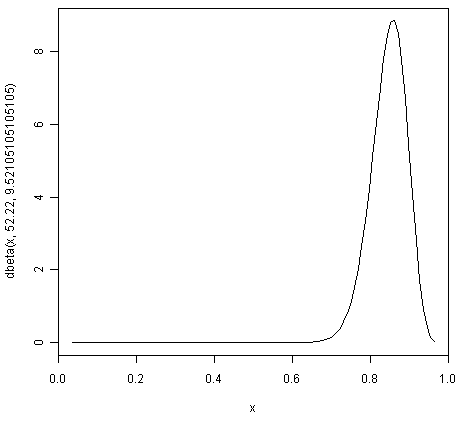
\includegraphics{image1.png}

Note that in the command above we use the ``dbeta()'' function to specify that
the density of a Beta(52.22,9.52105105105105) distribution.

We can see from the picture of the density for a Beta(52.22,9.52105105105105) distribution
that it represents our prior beliefs about the proportion of people who like chocolate
fairly well, as the peak of the distribution is at about 0.85, and the density lies
almost entirely between about 0.68 and 0.97.


\subsection{Calculating the Likelihood Function for a Proportion}
\label{src/bayesianstats:calculating-the-likelihood-function-for-a-proportion}
Say you want to estimate a proportion, and you have a small data set that you can use for this
purpose. For example, if you want to estimate the proportion of people who like chocolate, you
may have carried out a survey of 50 people, and found that 45 say that they like chocolate.

This small data set can be used to calculate the conditional p.m.f. (probability mass function)
of the proportion given the observed data. This is called the likelihood function. It represents
how likely the possible values of the proportion are, given the observed data.

If you want to estimate a proportion, and have a small data set, you can calculate the likelihood
function for the proportion using the function calcLikelihoodForProportion() below:

\begin{Verbatim}[commandchars=\\\{\}]
\PYG{o}{\textgreater{}} calcLikelihoodForProportion \PYG{o}{\textless{}-} \PYG{k+kr}{function}\PYG{p}{(}successes\PYG{p}{,} total\PYG{p}{)}
  \PYG{p}{\PYGZob{}}
     curve\PYG{p}{(}dbinom\PYG{p}{(}successes\PYG{p}{,}total\PYG{p}{,}x\PYG{p}{)}\PYG{p}{)} \PYG{c+c1}{\PYGZsh{} plot the likelihood}
  \PYG{p}{\PYGZcb{}}
\end{Verbatim}

The function calcLikelihoodForProportion() takes two input arguments: the number of successes
observed in the sample (eg. the number of people who like chocolate in the sample), and the
total sample size.

You can see that the likelihood function is being calculated using the Binomial distribution
(using the R ``dbinom()'' function). That is, the likelihood function is the probability
mass function of a B(total,successes) distribution, that is, of a Binomial distribution where the
we observe ``successes'' successes out of a sample of ``total'' observations in total.

For example, if we did a survey of 50 people, and found that 45 say they like chocolate, then
our total sample size is 50 and we have 45 ``successes''. We can calculate the likelihood
function for the proportion of people who like chocolate by typing:

\begin{Verbatim}[commandchars=\\\{\}]
\PYG{o}{\textgreater{}} calcLikelihoodForProportion\PYG{p}{(}\PYG{l+m}{45}\PYG{p}{,} \PYG{l+m}{50}\PYG{p}{)}
\end{Verbatim}

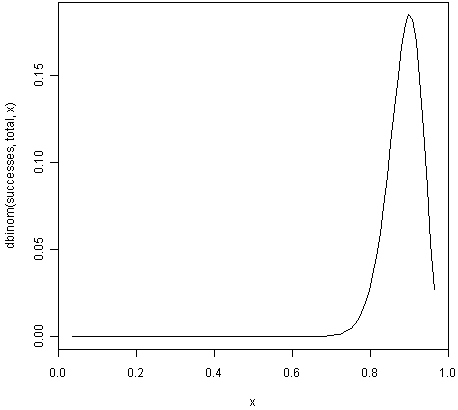
\includegraphics{image2.png}

You can see that the peak of the likelihood distribution is at 0.9, which is equal to the
sample mean (45/50 = 0.9). In other words, the most likely value of the proportion, given the
observed data, is 0.9.


\subsection{Calculating the Posterior Distribution for a Proportion}
\label{src/bayesianstats:calculating-the-posterior-distribution-for-a-proportion}
Say you are trying to estimate a proportion, and have a prior distribution representing
your beliefs about the value of that proportion. If you have collected some data, you
can also calculate the likelihood function for the proportion given the data.

However, after observing the data, you may wish to update the prior distribution for
the proportion, taking the data into consideration. That is, you may wish to calculate
the conditional distribution of the proportion given the data and the prior. This is is called
the posterior distribution for the proportion.

The posterior distribution ssummarises what is known about the proportion after the data
has been observed, and combines the information from the prior and the data.

In our example of estimating the proportion of people who like chocolate, we have a Beta(52.22,9.52) prior
distribution (see above), and have some data from a survey in which we found that 45 out of 50 people like
chocolate. We can calculate the posterior distribution for the proportion given the prior and data using
the calcPosteriorForProportion() function below (which I adapted from ``triplot'' in the LearnBayes
package):

\begin{Verbatim}[commandchars=\\\{\}]
\PYG{o}{\textgreater{}} calcPosteriorForProportion \PYG{o}{\textless{}-} \PYG{k+kr}{function}\PYG{p}{(}successes\PYG{p}{,} total\PYG{p}{,} a\PYG{p}{,} b\PYG{p}{)}
  \PYG{p}{\PYGZob{}}
     \PYG{c+c1}{\PYGZsh{} Adapted from triplot() in the LearnBayes package}
     \PYG{c+c1}{\PYGZsh{} Plot the prior, likelihood and posterior:}
     likelihood\PYGZus{}a \PYG{o}{=} successes \PYG{o}{+} \PYG{l+m}{1}\PYG{p}{;} likelihood\PYGZus{}b \PYG{o}{=} total \PYG{o}{-} successes \PYG{o}{+} \PYG{l+m}{1}
     posterior\PYGZus{}a \PYG{o}{=} a \PYG{o}{+} successes\PYG{p}{;}  posterior\PYGZus{}b \PYG{o}{=} b \PYG{o}{+} total \PYG{o}{-} successes
     theta \PYG{o}{=} seq\PYG{p}{(}\PYG{l+m}{0.005}\PYG{p}{,} \PYG{l+m}{0.995}\PYG{p}{,} length \PYG{o}{=} \PYG{l+m}{500}\PYG{p}{)}
     prior \PYG{o}{=} dbeta\PYG{p}{(}theta\PYG{p}{,} a\PYG{p}{,} b\PYG{p}{)}
     likelihood \PYG{o}{=} dbeta\PYG{p}{(}theta\PYG{p}{,} likelihood\PYGZus{}a\PYG{p}{,} likelihood\PYGZus{}b\PYG{p}{)}
     posterior  \PYG{o}{=} dbeta\PYG{p}{(}theta\PYG{p}{,} posterior\PYGZus{}a\PYG{p}{,} posterior\PYGZus{}b\PYG{p}{)}
     m \PYG{o}{=} max\PYG{p}{(}c\PYG{p}{(}prior\PYG{p}{,} likelihood\PYG{p}{,} posterior\PYG{p}{)}\PYG{p}{)}
     plot\PYG{p}{(}theta\PYG{p}{,} posterior\PYG{p}{,} type \PYG{o}{=} \PYG{l+s}{"}\PYG{l+s}{l"}\PYG{p}{,} ylab \PYG{o}{=} \PYG{l+s}{"}\PYG{l+s}{Density"}\PYG{p}{,} lty \PYG{o}{=} \PYG{l+m}{2}\PYG{p}{,} lwd \PYG{o}{=} \PYG{l+m}{3}\PYG{p}{,}
          main \PYG{o}{=} paste\PYG{p}{(}\PYG{l+s}{"}\PYG{l+s}{beta("}\PYG{p}{,} a\PYG{p}{,} \PYG{l+s}{"}\PYG{l+s}{,"}\PYG{p}{,} b\PYG{p}{,} \PYG{l+s}{"}\PYG{l+s}{) prior, B("}\PYG{p}{,} total\PYG{p}{,} \PYG{l+s}{"}\PYG{l+s}{,"}\PYG{p}{,} successes\PYG{p}{,} \PYG{l+s}{"}\PYG{l+s}{) data,"}\PYG{p}{,}
          \PYG{l+s}{"}\PYG{l+s}{beta("}\PYG{p}{,} posterior\PYGZus{}a\PYG{p}{,} \PYG{l+s}{"}\PYG{l+s}{,"}\PYG{p}{,} posterior\PYGZus{}b\PYG{p}{,} \PYG{l+s}{"}\PYG{l+s}{) posterior"}\PYG{p}{)}\PYG{p}{,} ylim \PYG{o}{=} c\PYG{p}{(}\PYG{l+m}{0}\PYG{p}{,} m\PYG{p}{)}\PYG{p}{,} col \PYG{o}{=} \PYG{l+s}{"}\PYG{l+s}{red"}\PYG{p}{)}
     lines\PYG{p}{(}theta\PYG{p}{,} likelihood\PYG{p}{,} lty \PYG{o}{=} \PYG{l+m}{1}\PYG{p}{,} lwd \PYG{o}{=} \PYG{l+m}{3}\PYG{p}{,} col \PYG{o}{=} \PYG{l+s}{"}\PYG{l+s}{blue"}\PYG{p}{)}
     lines\PYG{p}{(}theta\PYG{p}{,} prior\PYG{p}{,} lty \PYG{o}{=} \PYG{l+m}{3}\PYG{p}{,} lwd \PYG{o}{=} \PYG{l+m}{3}\PYG{p}{,} col \PYG{o}{=} \PYG{l+s}{"}\PYG{l+s}{green"}\PYG{p}{)}
     legend\PYG{p}{(}x\PYG{o}{=}\PYG{l+m}{0.8}\PYG{p}{,}y\PYG{o}{=}m\PYG{p}{,} c\PYG{p}{(}\PYG{l+s}{"}\PYG{l+s}{Prior"}\PYG{p}{,} \PYG{l+s}{"}\PYG{l+s}{Likelihood"}\PYG{p}{,} \PYG{l+s}{"}\PYG{l+s}{Posterior"}\PYG{p}{)}\PYG{p}{,} lty \PYG{o}{=} c\PYG{p}{(}\PYG{l+m}{3}\PYG{p}{,} \PYG{l+m}{1}\PYG{p}{,} \PYG{l+m}{2}\PYG{p}{)}\PYG{p}{,}
          lwd \PYG{o}{=} c\PYG{p}{(}\PYG{l+m}{3}\PYG{p}{,} \PYG{l+m}{3}\PYG{p}{,} \PYG{l+m}{3}\PYG{p}{)}\PYG{p}{,} col \PYG{o}{=} c\PYG{p}{(}\PYG{l+s}{"}\PYG{l+s}{green"}\PYG{p}{,} \PYG{l+s}{"}\PYG{l+s}{blue"}\PYG{p}{,} \PYG{l+s}{"}\PYG{l+s}{red"}\PYG{p}{)}\PYG{p}{)}
     \PYG{c+c1}{\PYGZsh{} Print out summary statistics for the prior, likelihood and posterior:}
     calcBetaMode \PYG{o}{\textless{}-} \PYG{k+kr}{function}\PYG{p}{(}aa\PYG{p}{,} bb\PYG{p}{)} \PYG{p}{\PYGZob{}} BetaMode \PYG{o}{\textless{}-} \PYG{p}{(}aa \PYG{o}{-} \PYG{l+m}{1}\PYG{p}{)}\PYG{o}{/}\PYG{p}{(}aa \PYG{o}{+} bb \PYG{o}{-} \PYG{l+m}{2}\PYG{p}{)}\PYG{p}{;} \PYG{k+kr}{return}\PYG{p}{(}BetaMode\PYG{p}{)}\PYG{p}{;} \PYG{p}{\PYGZcb{}}
     calcBetaMean \PYG{o}{\textless{}-} \PYG{k+kr}{function}\PYG{p}{(}aa\PYG{p}{,} bb\PYG{p}{)} \PYG{p}{\PYGZob{}} BetaMean \PYG{o}{\textless{}-} \PYG{p}{(}aa\PYG{p}{)}\PYG{o}{/}\PYG{p}{(}aa \PYG{o}{+} bb\PYG{p}{)}\PYG{p}{;} \PYG{k+kr}{return}\PYG{p}{(}BetaMean\PYG{p}{)}\PYG{p}{;} \PYG{p}{\PYGZcb{}}
     calcBetaSd   \PYG{o}{\textless{}-} \PYG{k+kr}{function}\PYG{p}{(}aa\PYG{p}{,} bb\PYG{p}{)} \PYG{p}{\PYGZob{}} BetaSd \PYG{o}{\textless{}-} sqrt\PYG{p}{(}\PYG{p}{(}aa \PYG{o}{*} bb\PYG{p}{)}\PYG{o}{/}\PYG{p}{(}\PYG{p}{(}\PYG{p}{(}aa \PYG{o}{+} bb\PYG{p}{)}\PYG{o}{\PYGZca{}}\PYG{l+m}{2}\PYG{p}{)} \PYG{o}{*} \PYG{p}{(}aa \PYG{o}{+} bb \PYG{o}{+} \PYG{l+m}{1}\PYG{p}{)}\PYG{p}{)}\PYG{p}{)}\PYG{p}{;} \PYG{k+kr}{return}\PYG{p}{(}BetaSd\PYG{p}{)}\PYG{p}{;} \PYG{p}{\PYGZcb{}}
     prior\PYGZus{}mode      \PYG{o}{\textless{}-} calcBetaMode\PYG{p}{(}a\PYG{p}{,} b\PYG{p}{)}
     likelihood\PYGZus{}mode \PYG{o}{\textless{}-} calcBetaMode\PYG{p}{(}likelihood\PYGZus{}a\PYG{p}{,} likelihood\PYGZus{}b\PYG{p}{)}
     posterior\PYGZus{}mode  \PYG{o}{\textless{}-} calcBetaMode\PYG{p}{(}posterior\PYGZus{}a\PYG{p}{,} posterior\PYGZus{}b\PYG{p}{)}
     prior\PYGZus{}mean      \PYG{o}{\textless{}-} calcBetaMean\PYG{p}{(}a\PYG{p}{,} b\PYG{p}{)}
     likelihood\PYGZus{}mean \PYG{o}{\textless{}-} calcBetaMean\PYG{p}{(}likelihood\PYGZus{}a\PYG{p}{,} likelihood\PYGZus{}b\PYG{p}{)}
     posterior\PYGZus{}mean  \PYG{o}{\textless{}-} calcBetaMean\PYG{p}{(}posterior\PYGZus{}a\PYG{p}{,} posterior\PYGZus{}b\PYG{p}{)}
     prior\PYGZus{}sd        \PYG{o}{\textless{}-} calcBetaSd\PYG{p}{(}a\PYG{p}{,} b\PYG{p}{)}
     likelihood\PYGZus{}sd   \PYG{o}{\textless{}-} calcBetaSd\PYG{p}{(}likelihood\PYGZus{}a\PYG{p}{,} likelihood\PYGZus{}b\PYG{p}{)}
     posterior\PYGZus{}sd    \PYG{o}{\textless{}-} calcBetaSd\PYG{p}{(}posterior\PYGZus{}a\PYG{p}{,} posterior\PYGZus{}b\PYG{p}{)}
     print\PYG{p}{(}paste\PYG{p}{(}\PYG{l+s}{"}\PYG{l+s}{mode for prior="}\PYG{p}{,}prior\PYGZus{}mode\PYG{p}{,}\PYG{l+s}{"}\PYG{l+s}{, for likelihood="}\PYG{p}{,}likelihood\PYGZus{}mode\PYG{p}{,}\PYG{l+s}{"}\PYG{l+s}{, for posterior="}\PYG{p}{,}posterior\PYGZus{}mode\PYG{p}{)}\PYG{p}{)}
     print\PYG{p}{(}paste\PYG{p}{(}\PYG{l+s}{"}\PYG{l+s}{mean for prior="}\PYG{p}{,}prior\PYGZus{}mean\PYG{p}{,}\PYG{l+s}{"}\PYG{l+s}{, for likelihood="}\PYG{p}{,}likelihood\PYGZus{}mean\PYG{p}{,}\PYG{l+s}{"}\PYG{l+s}{, for posterior="}\PYG{p}{,}posterior\PYGZus{}mean\PYG{p}{)}\PYG{p}{)}
     print\PYG{p}{(}paste\PYG{p}{(}\PYG{l+s}{"}\PYG{l+s}{sd for prior="}\PYG{p}{,}prior\PYGZus{}sd\PYG{p}{,}\PYG{l+s}{"}\PYG{l+s}{, for likelihood="}\PYG{p}{,}likelihood\PYGZus{}sd\PYG{p}{,}\PYG{l+s}{"}\PYG{l+s}{, for posterior="}\PYG{p}{,}posterior\PYGZus{}sd\PYG{p}{)}\PYG{p}{)}
  \PYG{p}{\PYGZcb{}}
\end{Verbatim}

To use the ``calcPosteriorForProportion()'' function, you will first need to copy and paste it into R.
It takes four arguments: the number of successes and total sample size in your data set, and the
a and b values for your Beta prior.

For example, to estimate the proportion of people who like chocolate, you had a Beta(52.22,9.52) prior
and had observed in a survey that 45 out of 50 people like chocolate. Therefore, the number of successes
is 45, the sample size is 50, and a and b for the prior are 52.22 and 9.52 respectively. Therefore, we
can calculate the posterior for the proportion of people who like chocolate, given the data and prior, by typing:

\begin{Verbatim}[commandchars=\\\{\}]
\PYG{o}{\textgreater{}} calcPosteriorForProportion\PYG{p}{(}\PYG{l+m}{45}\PYG{p}{,} \PYG{l+m}{50}\PYG{p}{,} \PYG{l+m}{52.22}\PYG{p}{,} \PYG{l+m}{9.52}\PYG{p}{)}
  \PYG{p}{[}\PYG{l+m}{1}\PYG{p}{]} \PYG{l+s}{"}\PYG{l+s}{mode for prior= 0.857381988617342 , for likelihood= 0.9 , for posterior= 0.876799708401677"}
  \PYG{p}{[}\PYG{l+m}{1}\PYG{p}{]} \PYG{l+s}{"}\PYG{l+s}{mean for prior= 0.845804988662132 , for likelihood= 0.884615384615385 , for posterior= 0.870055485949526"}
  \PYG{p}{[}\PYG{l+m}{1}\PYG{p}{]} \PYG{l+s}{"}\PYG{l+s}{sd for prior= 0.0455929848904483 , for likelihood= 0.0438847130123102 , for posterior= 0.0316674748482802"}
\end{Verbatim}

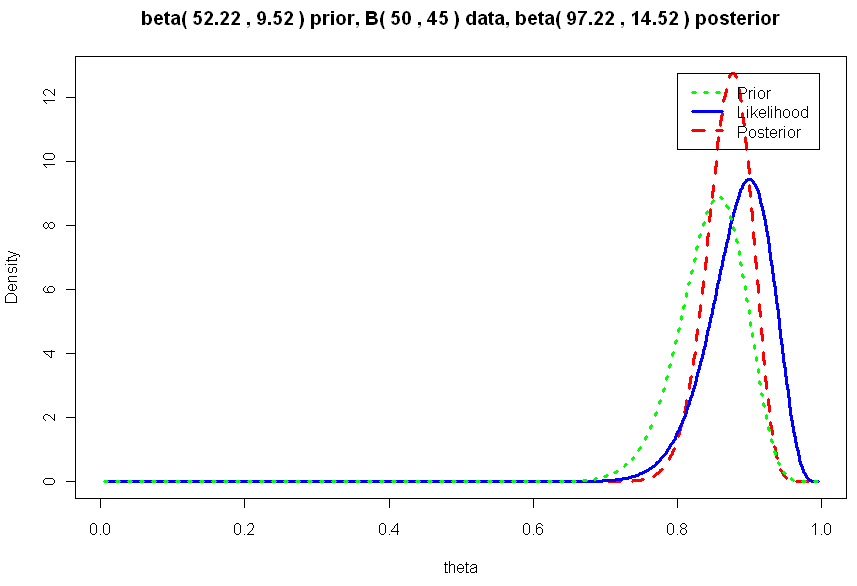
\includegraphics{image4.png}

Since the prior and posterior are distributions, the area under their densities is 1.
The likelihood has been scaled so that the area underneath it is also 1, so that it is
easy to compare the likelihood with the prior and posterior.

Therefore, the prior and likelihood curves should look the same shape as those plotted
before (see above), but the y-axis scale is different for the likelihood scale compared
to the plot made using calcLikelihoodForProportion() above.

Note that the peak of the posterior always lies somewhere between the peaks of the prior and the
likelihood, because it combines information from the prior and the likelihood (which is based on the data).

In our example of estimating the proportion of people who like chocolate,
the peak of the posterior is roughly half-way between the peaks of the likelihood and prior,
indicating that the prior and the data contribute roughly equally to the posterior.


\section{Links and Further Reading}
\label{src/bayesianstats:links-and-further-reading}
Here are some links for further reading.

For a more in-depth introduction to R, a good online tutorial is
available on the ``Kickstarting R'' website,
\href{http://cran.r-project.org/doc/contrib/Lemon-kickstart/}{cran.r-project.org/doc/contrib/Lemon-kickstart}.

There is another nice (slightly more in-depth) tutorial to R
available on the ``Introduction to R'' website,
\href{http://cran.r-project.org/doc/manuals/R-intro.html}{cran.r-project.org/doc/manuals/R-intro.html}.

To learn about Bayesian Statistics, I would highly recommend the book ``Bayesian
Statistics'' (product code M249/04) by the Open University, available from \href{http://www.ouw.co.uk/store/}{the Open University Shop}.

There is a book available in the ``Use R!'' series on using R for multivariate analyses,
\href{http://www.springer.com/statistics/statistical+theory+and+methods/book/978-0-387-92297-3}{Bayesian Computation with R} by Jim Albert.


\section{Acknowledgements}
\label{src/bayesianstats:acknowledgements}
Many of the examples in this booklet are inspired by examples in the excellent Open University book,
``Bayesian Statistics'' (product code M249/04),
available from \href{http://www.ouw.co.uk/store/}{the Open University Shop}.


\section{Contact}
\label{src/bayesianstats:contact}
I will be grateful if you will send me (\href{http://www.sanger.ac.uk/research/projects/parasitegenomics/}{Avril Coghlan}) corrections or suggestions for improvements to
my email address \href{mailto:alc@sanger.ac.uk}{alc@sanger.ac.uk}


\section{License}
\label{src/bayesianstats:license}
The content in this book is licensed under a \href{http://creativecommons.org/licenses/by/3.0/}{Creative Commons Attribution 3.0 License}.


\chapter{Acknowledgements}
\label{index:acknowledgements}
Thank you to Noel O'Boyle for helping in using Sphinx, \href{http://sphinx.pocoo.org}{http://sphinx.pocoo.org}, to create
this document, and github, \href{https://github.com/}{https://github.com/}, to store different versions of the document
as I was writing it, and readthedocs, \href{http://readthedocs.org/}{http://readthedocs.org/}, to build and distribute
this document.


\chapter{Contact}
\label{index:contact}
I will be very grateful if you will send me (\href{http://www.sanger.ac.uk/research/projects/parasitegenomics/}{Avril Coghlan}) corrections or suggestions for improvements to
my email address \href{mailto:alc@sanger.ac.uk}{alc@sanger.ac.uk}


\chapter{License}
\label{index:license}
The content in this book is licensed under a \href{http://creativecommons.org/licenses/by/3.0/}{Creative Commons Attribution 3.0 License}.



\renewcommand{\indexname}{Index}
\printindex
\end{document}
